\documentclass[11pt,a4paper]{article}
 
\usepackage{polski}
\usepackage[utf8]{inputenc} %utf-8 żeby nie było problemów z przenoszeniem między windowsem a linuxem
\usepackage{graphicx}
\usepackage{listings}
\usepackage{indentfirst}
\usepackage{rotating}

%lokalne makro na komendę
\newcommand{\HRule}{\rule{\linewidth}{0.5mm}}

\setlength\parindent{24pt}
\oddsidemargin=20pt
\textwidth=420pt



 
\begin{document}

%strona tytułowa
\begin{titlepage}
\begin{center}
%nagłówek uczelni
\textsc{\LARGE Politechnika Warszawska}\\[0.5cm]
\textsc{\Large Wydział Elektroniki i Technik Informacyjnych}\\
\textsc{\Large Instytut Automatyki i Informatyki Stosowanej}\\[1.5cm]

\textsc{\Large Praca inżynierska} \\[0.5cm]
%tytuł między kreskami
\HRule \\[0.4cm]
{ \huge \bfseries Generator raportów z baz danych w technologii XSL-FO  bazujący na wzorcach \\[0.4cm]}
\HRule \\[1.5cm]

%autor
\begin{minipage} {0.4\textwidth}
\begin{flushleft} \large
\emph{Autor:}\\
 Maciej Kucharski 
\end{flushleft}
\end{minipage}
%promotor
\begin{minipage} {0.4\textwidth}
\begin{flushright} \large

\emph{Opiekun:}\\
doc. dr inż. Tomasz Traczyk

\end{flushright}
\end{minipage}	
\vfill
\large Semestr 14Z

	\end{center}
\end{titlepage}
 
\tableofcontents
\newpage

%Wstęp
\section{Wstęp} \label{sec:wst}
Obecnie bazy danych wykorzystywane są powszechnie. Niemal każde przedsiębiorstwo dysponujące przynajmniej podstawową infrastrukturą informatyczną wykorzystuje w swoich działaniach bazę danych. Dane zgromadzone w takiej bazie danych często muszą być przedstawiane, np. zarządowi przedsiębiorstwa, bądź udostępniane publicznie w przypadku instytucji publicznych. Zwykła, surowa tabela będąca wynikiem działania zapytania \emph{SQL} nie jest wystarczająca dla takich zastosowań ze względu na jej ubogi wygląd oraz kiepską czytelność.  Samo pobieranie raportowanych danych z bazy również jest problematyczne ze względu na konieczność znajomości języka \emph{SQL}. 

Funkcjonalny z punktu widzenia biznesu system raportowy powinien spełniać pewne wymagania:
\begin{itemize}
	\item umożliwienie stosowania własnych wzorców wyglądu raportu (tzw. \emph{layout}),
	\item minimalizacja wymaganej do obsługi ilości wiedzy informatycznej ,
	\item umożliwienie generowania raportów w formacie \emph{PDF} w celu uniknięcia problemów wynikających z innego wyświetlania na różnych platformach systemowych.
\end{itemize}

Na rynku dostępna jest cała gama narzędzi spełniających powyższe wymagania w mniejszym lub większym stopniu. Najlepszym przykładem jest \emph{Oracle BI Publisher}, który spełnia wszystkie wyżej postawione wymagania, jednak konieczność corocznego ponoszenia niemałych kosztów wynikających z opłat licencyjnych sprawia, że jest on w zasięgu niewielu organizacji.

Alternatywą jest darmowy \emph{Oracle Application Express}, zwany również \emph{ApEx'em}, instalujący się wraz z bazą danych \emph{Oracle}. Standardowo generowane przez \emph{ApEx} raporty nie są zbyt zaawansowane graficznie. Celem niniejszej pracy jest opracowanie rozwiązań zwiększających jego możliwości.

\emph{ApEx} umożliwia skorzystanie z zewnętrznego serwera wydruków do tworzenia raportów w formacie \emph{PDF}. W tym celu potrzebny jest raport w postaci \emph{XSL-FO}. Postać tę można uzyskać poprzez zastosowanie transformacji \emph{XSLT} do danych w formacie \emph{XML}. Jest to jednak kłopotliwe w przypadku ręcznego tworzenia arkuszy transformacji \emph{XSLT}, gdyż zmiany we wzorcu wyglądu raportu pociągają za sobą konieczność wykorzystania wiedzy eksperckiej w celu modyfikacji arkusza \emph{XSLT}.

\bigskip
W ramach pracy przygotowano:
\begin{itemize}
	\item narzędzie generujące arkusz przekształceń \emph{XSLT} na podstawie danych wejściowych i wzorca wyglądu raportu,
	\item przykładową konfigurację \emph{ApEx},
	\item przykładowe wzorce wyglądu raportu w celu demonstracji.
\end{itemize}


\newpage

\section{Raporty} \label{sec:teoria}
Raport jest standardową formą dokumentu biznesowego, który służy do logicznej prezentacji informacji jakościowych oraz ilościowych.
 Raporty, w zależności od swojego zastosowania, mogą zawierać różne informacje i być przeznaczone dla różnych grup odbiorców. Układ wizualny raportu powinien być dostosowany do odbiorcy: raport przygotowany dla celów operacyjnych nie musi mieć atrakcyjnej szaty graficznej, w przeciwieństwie do raportu przeznaczonego dla kierownictwa organizacji, bądź wglądu publicznego. 

Funkcjami raportów są np. podsumowywanie kluczowych wskaźników biznesu, prezentacja miar biznesowych w oparciu o rozmaite statystyki, czy ocena wydajności biznesowej, umożliwiająca szybką weryfikację stopnia realizacji strategicznych celów przedsiębiorstwa. Ze względu na swoje funkcje, raporty należą do najważniejszych dokumentów, którymi dysponuje organizacja. 
Za raport może być uznany każdy dokument prezentujący jakieś dane w ustandaryzowany sposób, jednak w ramach niniejszej pracy ograniczono się do podstawowych typów raportów najczęściej występujących w praktyce. Zostaną one zaprezentowane w dalszej części rozdziału.

\subsection{Raport typu \emph{master-detail}} \label{teoria:md}
Ten typ raportu służy prezentacji wartości pełniących funkcję nadrzędnych względem innych oraz szczegóły aktualnie wybranej pozycji. Ten typ raportu może być zastosowany przy występowaniu związków typu jeden-do-wielu. Najlepszym przykładem raportu tego typu jest powszechnie występujący dokument, jakim jest faktura. 

Zarówno obszar nadrzędny, jak i podrzędny może być listą lub drzewem pozycji, co umożliwia wprowadzenie wielu stopni podrzędności. Obszar podrzędny zwykle jest prezentowany pod obszarem nadrzędnym lub obok niego. Przykładem może być wspomniana uprzednio faktura prezentująca spis pozycji wchodzących w skład zamówienia lub spis pracowników zatrudnionych w konkretnym dziale spółki. Przykładowa faktura zaprezentowana jest na rysunku \ref{img:faktura}. Dane klienta i numer faktury są uznawane za dane nadrzędne, zaś pozycje występujące na fakturze -- podrzędne. 

%źródło
%http://www.infakt.pl/images/icons-for_articles/grafiki/faktura_vat_pdf.png
\begin{figure}[h]
\centering
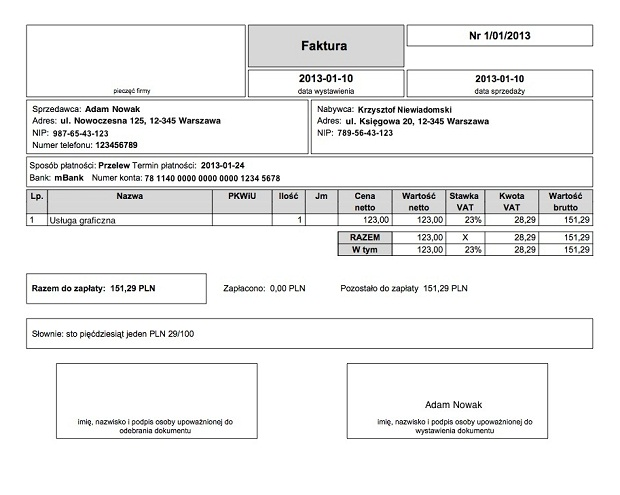
\includegraphics[scale=0.80]{faktura_vat_pdf}
\caption{Faktura jako przykład raportu \emph{master-detail}}
\label{img:faktura}
\end{figure}

\subsection{Raport z grupami łamiącymi (\emph{break-groups})} \label{teoria:bg}
Głównym celem tego typu raportu jest zwiększenie jego czytelności. Polega na podziale wierszy trafiających do raportu na grupy o jednakowych wartościach w wyróżnionych kolumnach. Każda z takich grup może zostać odpowiednio obsłużona, np. poprzez opatrzenie ich nagłówkami, wyliczenie dla nich podsumowań itp. Taka struktura umożliwia dość elastyczną prezentację tych samych danych. Grupy łamiące mogą być zastosowane w innych typach raportów, np. wspomnianym wyżej raporcie \emph{master-detail}. Na rysunku \ref{img:bg} zaprezentowany jest przykład raportu wykorzystującego grupy łamiące. Dane przedstawione na nim są zgrupowane według wartości zawartych w pierwszej kolumnie.
%źródło
%http://docs.oracle.com/cd/E17904_01/bi.1111/b32122/img/grp1col_lft1_out1.gif
\begin{figure}[h]
\centering
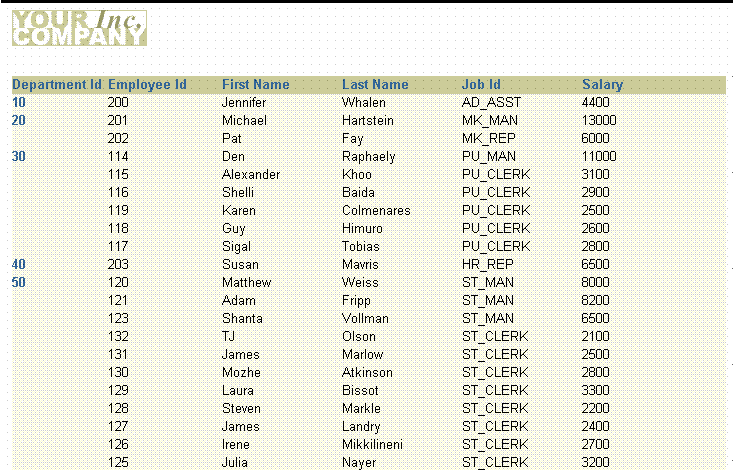
\includegraphics[scale=0.7]{grp1col_lft1_out1}
\caption{Przykład raportu wykorzystującego grupy łamiące}
\label{img:bg}
\end{figure}

\subsection{Raport macierzowy (krzyżowy) } \label{teoria:ct}
Raport macierzowy jest wykorzystywany do prezentacji związków między dwoma wymiarami. Raporty tego typu są często wykorzystane do analizy różnego rodzaju ankiet. Raport taki przedstawia związek między dwoma zmiennymi, tym samym ułatwiając znalezienie zależności między nimi. Struktura raportu tego typu może być porównana do wyglądu tabeli przestawnej z programu \emph{MS Excel}. W szczególności w ten sposób można raportować dane między którymi nie ma jawnej zależności. Przykład raportu macierzowego jest przedstawiony na rysunku \ref{img:ct}. Prezentuje on sprzedaż pewnych produktów w poszczególnych latach. 

%źrodło: http://doc.windev.com/en-US/images/image.awp?langid=3&name=etatTableaucroise3.gif&-1373238303
\begin{figure}[h]
\centering
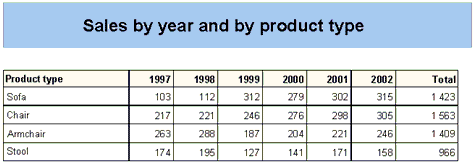
\includegraphics[scale=1]{crosstab_report}
\caption{Przykład raportu macierzowego}
\label{img:ct}
\end{figure}

\newpage

%Narzędzia
\section{Wykorzystane narzędzia i technologie} \label{sec:tools}
Pomimo pozornej prostoty raportowania, w przyjętym rozwiązaniu wykorzystanych jest wiele rozmaitych standardów oraz już istniejących narzędzi. Najważniejsze z nich zostaną pokrótce przedstawione w następujących podrozdziałach.

\subsection{Oracle Application Express (ApEx)} \label{tools:apex}
Oracle Application Express, zwany również ApEx'em, jest darmowym narzędziem instalującym się wraz z bazą danych firmy \emph{Oracle}. Umożliwia ono zarówno szybkie tworzenie strony raportowych, jak i bardziej skomplikowanych aplikacji zawierających nietrywialną logikę.

 Posiada wbudowany kreator zapytań \emph{SQL}, dzięki czemu osoba z minimalnym przygotowaniem informatycznym jest w stanie określić odpowiednie zapytanie pobierające dane z bazy. \emph{ApEx} nie posiada jednak wbudowanego mechanizmu pozwalającego na tworzenie wydruków w formacie \emph{PDF}. W tym celu należy skorzystać z zewnętrznego narzędzia. Jednym z nich może być Oracle BI Publisher, jednak nie jest to narzędzie tanie, a poza tym samo w sobie jest kompletnym systemem raportowym, a zatem w przypadku jego posiadania stosowanie ApExa jest zbędne. Alternatywą jest wykorzystanie \emph{APEX Listenera} wraz z wbudowanym w niego \emph{FOP}. \emph{FOP} jest darmowym narzędziem pozwalającym na generowanie plików w formacie \emph{PDF} szerzej omówionym w rozdziale \ref{tools:fop}. Poglądowy schemat wykorzystania FOP przez \emph{ApExa} za pośrednictwem \emph{APEX Listnera} jest zaprezentowany na rysunku \ref{img:apex_fop}. Pierwszym krokiem do wygenerowania raportu jest zainicjowane tego procesu przez użytkownika końcowego za pośrednictwem \emph{APEX Listnera}. Przekazuje on żądanie do bazy danych, a ta z kolei zwraca w odpowiedzi dane w formacie XML oraz wzorzec wyglądu raportu, a dokładniej transformację XSLT odpowiadającą za stworzenie dokumentu w formacie XSL-FO poprzez przekształcenie danych w XML. Następnie wewnątrz \emph{APEX Listenera} za pomocą wbudowanego \emph{FOP} wykonywana jest transformacja \emph{XSLT}. W efekcie dane zostają przekształcone do postaci \emph{XSL-FO}, z której możliwe jest utworzonie raportu w formacie \emph{PDF}. Ten z kolei jest zwracany użytkownikowi końcowemu. 

%rozmieści się samo gdzieś
\begin{figure}[h]
\centering
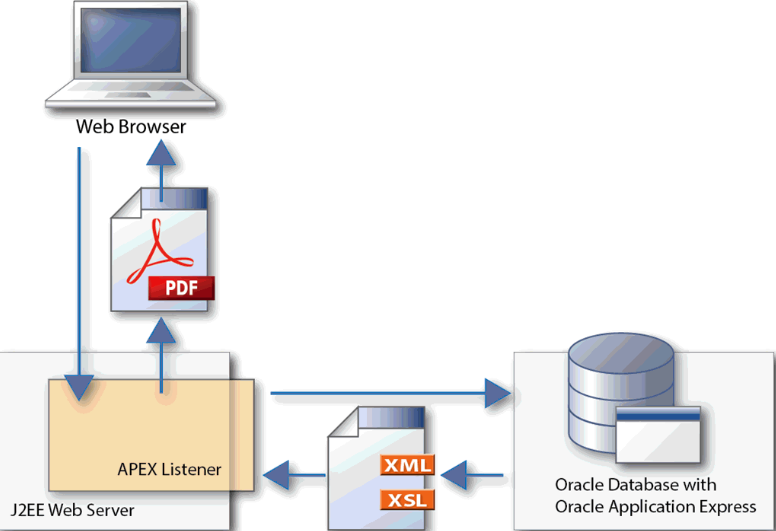
\includegraphics[scale=0.5]{apex_listener_fop}
\caption{Wykorzystanie FOP przez Oracle Application Express}
\label{img:apex_fop}
\end{figure}

Ręczne tworzenie arkuszy XSLT dla potrzeb raportów jest jednak problematyczne. Zmiany we wzorcu wyglądu raportu pociągają za sobą konieczność dokonania zmian w transformacji XSLT. W przypadku drobnych zmian, takich jak np. zmiana marginesu bądź rozmiaru pewnego elementu problem nie jest jeszcze tak duży, jednak w przypadku konieczności np. dodania nowego elementu konieczne jest już skorzystanie ze specjalistycznej wiedzy. Ponadto stworzenie nowego wzorca od podstaw jest problematyczne dla osoby nie posiadającej wymaganych kompetencji.

W ramach niniejszej pracy zostały opracowane rozwiązania, które umożliwią sprawne raportowanie z wykorzystaniem \emph{ApExa} użytkownikom biznesowym, nie posiadającym wymaganej wiedzy informatycznej. Proponowane rozwiązanie to wykorzystanie dodatkowego narzędzia, które wyręczy użytkownika końcowego w przygotowaniu transformacji XSLT przekształcającej dane w formacie XML w postać XSL-FO.

Ponadto \emph{ApEx} umożliwia wywołanie zewnętrznych usług, zgodnych ze standardem \emph{RESTful}, dzięki czemu może zostać wykorzystany do stworzenia graficznego interfejsu wywołującego narzędzie opracowane w ramach pracy.

\subsection{XSLT} \label{tools:xslt}
XSLT (\emph{eXtensible Stylesheet Language Transformations} to oparty na XML język służący do przekstałcania jednych dokumentów w formacie XML na dowolne inne zgodnie z zadanymi regułami. Jest podzbiorem szerszej specyfikacji określanej jako XSL. Transformacje XSLT zapisywane są w dokumentach XML z wykorzystaniem specjalnej przestrzeni nazw. Ze względu na dużą siłę wyrazu, łatwość implementacji oraz powszechne stosowanie XML, XSLT jest szeroko stosowane w różnych rodzajach oprogramowania. Ze względu na fakt, że współczesne przeglądarki internetowe posiadają wbudowane procesory XSLT, najczęstszym jego zastosowaniem jest transformacja dokumentów XML w celu wyświetlenia w przeglądarce WWW. Rysunek \ref{img:xslt} prezentuje poglądowy schemat zastosowania XSLT. W ramach niniejszej pracy język XSLT jest stosowany do przekształcenia pliku XML w postać zgodną ze specyfikacją XSL-FO, co umożliwi stworzenie pliku z raportem w formacie PDF przez FOP.
\begin{figure}[h]
\centering
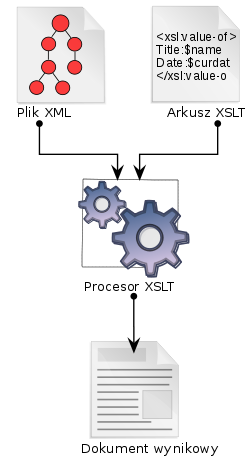
\includegraphics[scale=0.5]{xslt}
\caption{Schemat poglądowy zastosowania XSLT}
\label{img:xslt}
\end{figure}

\subsection{XSL-FO} \label{tools:xslfo}
XSL Formatting Objects to wykorzystujący XML język stosowany do formatowania dokumentów. Jest podzbiorem szerszej specyfikacji XSL. Dokumenty XSL-FO są zapisywane w XML z wykorzystaniem specjalnej przestrzeni nazw. Główną ideą powstania tej specyfikacji jest fakt, że w przeciwieństwie do HTML, czy XHTML, dokumenty XML nie posiadają wbudowanego układu wizualnego. XSL-FO jest językiem, który może zostać użyty do nadania dokumentowi XML układu na stronie, kolorów, czcionek itd. z przeznaczeniem wyniku dla różnych mediów, jak np. ekranu lub drukarki. W tym sensie pełni funkcję podobną do stylów CSS, jednak jest bardziej elastyczny i daje większe możliwości, zwłaszcza jeśli chodzi np. o stronicowanie i przewijanie. Główną różnicą między XSL-FO, a CSS jest fakt, że informacje o układzie wizualnym są zawarte w tym samym dokumencie, co dane. Oddzielenie danych od stylu można uzyskać np. przez zastosowanie transformacji XSLT do danych w XML.

\subsection{Apache FOP} \label{tools:fop}
Apache FOP (\emph{Formatting Objects Processor}) jest najpopularniejszym procesorem obiektów formatujących. Jest to darmowy program napisany w języku \emph{Java}, który konwertuje pliki zapisane w formacie XSL-FO na pliki w formacie PDF lub innych drukowalnych, m.in. RTF czy PostScript. FOP umożliwia również przetwarzanie danych w formacie XML przy użyciu odpowiednich transformacji XSLT. Najnowsza stabilna wersja nie pokrywa w pełni specyfikacji XSL-FO 1.1, lecz najważniejsze elementy są wspierane.

FOP może być wykorzystywany zarówno jako niezależna aplikacja uruchamiana np. z wiersza poleceń, jak i biblioteka Javy, co umożliwia wykorzystanie w dowolnej aplikacji przeznaczonej do uruchamiania w środowisku maszyny wirtualnej Javy (\emph{JVM}). Dodatkowo, wraz z instalacją ApExa dostarczane jest archiwum \emph{war} zawierające specjalnie przygotowaną wersję FOP przeznaczoną do uruchamiania na kontenerze serwletów. Domyślna konfiguracja nie wspiera jednak stosowania narodowych czcionek, np. polskich znaków, jednak jest to możliwe po zastosowaniu pewnych zmian w konfiguracji \emph{FOP}. 

W ramach pracy FOP jest wykorzystywany do generowania plików w formacie PDF.

\subsection{SVG} \label{tools:svg}
SVG (\emph{Scalable Vector Graphics}) to bazujący na XML format do zapisu dwuwymiarowej grafiki wektorowej. Jest to otwarty standard utworzony przez organizację W3C. Standard jest powszechnie wspierany przez współczesne przeglądarki internetowe, z myślą o których powstał. Może jednak być również wykorzystywany jako niezależny od platformy systemowej format grafiki wektorowej. Za pomocą SVG można tworzyć zarówno statyczne grafiki, jak i animacje.

Plik zawierający grafikę SVG może być utworzony i edytowany za pomocą dowolnego edytora tekstu, jednak wygodniejsze jest zastosowanie do tego celu dedykowanego oprogramowania. Polecanym do tego celu programem jest darmowy \emph{InkScape}. Umożliwia on utworzenie grafiki bez wnikania w techniczne aspekty specyfikacji SVG i generuje odpowiadający jej dokument XML.

W ramach pracy standard SVG jest wykorzystywany do zapisu wzorca wyglądu raportu. 

\subsection{Groovy} \label{tools:groovy}
\emph{Groovy} to obiektowy język programowania uruchamiany w środowisku maszyny wirtualnej \emph{Javy}, umożliwiający stosowanie dynamicznego typowania zmiennych. W \emph{Groovy} dozwolone jest również stosowanie tzw. domknięć (\emph{closure}), dzięki czemu możliwe jest programowanie funkcyjne oraz sprawne operowanie na kolekcjach. 

Oferowane przez \emph{Groovy} rozwiązania umożliwiają znacznie prostsze niż przy wykorzystaniu wyrażeń \emph{XPath} operowanie drzewem XML, co jest głównym powodem wykorzystania tej technologii w ramach pracy.

W ramach niniejszej pracy język programowania \emph{Groovy} został wykorzystany do sformułowania logiki odpowiedzialnej za generowanie arkuszy transformacji XSLT na podstawie danych zapisanych w formacie XML oraz wzorca wyglądu raportu zapisanego w SVG, czyli w istocie również XML. 

\subsection{Apache Maven} \label{tools:maven}
Apache Maven to narzędzie służące wspomaganiu procesu tworzenia oprogramowania. Dzięki zastosowaniu wtyczek, możliwości narzędzia są bardzo duże. W ramach pracy Maven jest wykorzystany głównie w trzech celach: 
\begin{itemize}
\item zarządzanie zależnościami, tj. automatyczne pobieranie niezbędnych bibliotek we właściwej wersji,
\item umożliwienie stosowania \emph{Groovy} w połączeniu z \emph{Javą},
\item automatyczne budowanie paczki z oprogramowaniem.
\end{itemize} 

W ramach pracy przewidziane są dwa rodzaje paczek. Pierwsza to archiwum \emph{jar} służące uruchomieniu np. z wiersza poleceń. Takie archiwum zawiera plik \textbf{\emph{MANIFEST.MF}}, którego ręczne tworzenie byłoby problematyczne. Wykorzystanie Mavena pozwala na jego automatyczne wygenerowania oraz dodatkowo skopiowania wszystkich bibliotek niezbędnych do uruchomienia. Drugi typ paczki to archiwum \emph{war} przeznaczone do uruchomienia na kontenerze serwletów. Archiwum to posiada tzw. deskryptor, który może być automatycznie wygenerowany przez Mavena.

\newpage


%Koncepcja
\section{Proponowane rozwiązanie problemu} \label{sec:solution}
\subsection{Ogólna koncepcja} \label{solution:koncept}
Głównym problemem przy wykorzystaniu ApExa jest konieczność tworzenia nowych arkuszy transformacji XSLT przy zmianach wzorca wyglądu raportu. Przy wykorzystaniu przez biznes jest to niedopuszczalne. W związku z tym w ramach pracy zostało przygotowane narzędzie mające na celu rozwiązanie tego problemu. Jego głównym przeznaczeniem jest wspieranie ApEx'a w zakresie generowania arkuszy transformacji XSLT na podstawie danych wejściowych w XML oraz wzorca wyglądu raportu w SVG. Arkusz ten może być wykorzystany do przekształcenia pliku XML z danymi w plik w formacie XSL-FO. Ten z kolei może zostać wysłany do FOP, co skutkuje utworzeniem raportu\\w formacie PDF.

\subsection{Dane wejściowe} \label{solution:data}
Dane przeznaczone do raportu zapisane są w formacie XML. Ponieważ dane pochodzą z ApExa, możliwe jest przyjęcie założeń odnośnie ich struktury. Ogólna struktura jest przedstawiona na listingu \ref{rap:apex}. Element REGION jest opcjonalny i może nie wystąpić. Wpis zawierający informacje zawarte w pojedynczym wierszu zawarte są w strukturze znacznika ROW. W nim z kolei znajdują się informacje dotyczące poszczególnych kolumn. Nazwa kolumny jest taka sama jak nazwa znacznika, zaś wartość odpowiadająca węzłowi to wartość konkretnej danej.

\lstset{language=XML}
\begin{lstlisting}[frame=single,caption=Ogólna postać dokumentu XML z danymi pochodzącymi z ApExa,label=rap:apex]
<?xml version="1.0" encoding="UTF-8"?>
<DOCUMENT>
 <REGION ID="">
  <ROWSET>
   <ROW>
    <KOLUMNA1>...</KOLUMNA1>
    <KOLUMNA2>...</KOLUMNA2>
       ...	
   </ROW>
   <ROW>....</ROW>
  </ROWSET>
 </REGION>
</DOCUMENT>
\end{lstlisting}

Ponadto w pliku danych mogą zostać przekazane dodatkowe informacje. Mogą to być np. informacje o zalogowanym użytkowniku, sesji, identyfikator aplikacji, data itp. Można również przekazać inne informacje znajdujące się w pewnym miejscu na stronie w ApExie. Jest to tzw. \emph{region}. Wtedy dodawany jest znacznik REGION. Fakt ten jest wykorzystywany do przekazania informacji ,,nadrzędnych" przy wyborze raportu typu \emph{master-detail}. Format danych ,,nadrzędnych" jest zaprezentowany na listingu \ref{rap:master}. Dane te zawarte są w strukturze głównego znacznika DOCUMENT. Litera X w widocznym przykładzie jest w rzeczywistości numerem strony w ApEx'ie, na której znajduje się owa dana. Litera P występuje zawsze. 

\lstset{language=XML}
\begin{lstlisting}[frame=single,caption=Format danych typu \emph{master},label=rap:master]
<?xml version="1.0" encoding="UTF-8"?>
<DOCUMENT>
 <PX_DANA1>...</PX_DANA1>
 <PX_DANA2>...</PX_DANA2>
 ...
</DOCUMENT>
\end{lstlisting}

Dodatkowym założeniem, mającym na celu uproszczenie stosowania grup łamiących w raportach, jest wymaganie, by zapytanie \emph{SQL} pobierające dane do raportu posiadało klauzulę \emph{ORDER BY} sortującą dane według odpowiednich kolumn. Rzeczywisty przykład danych wejściowych jest przedstawiony na listingu \ref{rap:complete}. Przedstawia on również sposób reprezentacji kolumn zawierających pustą wartość. 

\lstset{language=XML}
\begin{lstlisting}[frame=single,caption=Przykładowe dane,label=rap:complete]
<?xml version="1.0" encoding="UTF-8"?>
<DOCUMENT>
 <P8_DEPTNAME>Accounting</P8_DEPTNAME>
 <P8_DESCR>Department description</P8_DESCR>
   <ROWSET>
    <ROW>
      <JOB>PRESIDENT</JOB>
      <ENAME>KING</ENAME>
      <HIREDATE>11/17/1981</HIREDATE>
      <SAL>5000</SAL>
      <COMM/>
      <MGR/>
    </ROW>
   </ROWSET>
</DOCUMENT>
\end{lstlisting}

\subsection{Wzorzec wyglądu raportu} \label{solution:layout}
Wzorzec wyglądu raportu jest zapisany w formacie SVG, jak zostało to zaznaczone w rozdziale \ref{tools:svg}. Specyfikacja SVG zawiera bardzo dużo elementów. W ramach pracy nie byłoby możliwe pełne wsparcie specyfikacji, zatem przyjęto pewne ograniczenia. Wspieranymi elementami jest stały tekst, grafika (np. logo organizacji) oraz prostokąty jako pola danych, a zatem typowe komponenty wchodzące w skład raportu.

Kolejne założenie upraszczające dotyczy reprezentacji tabeli. W SVG nie występuje specjalna konstrukcja służąca do tworzenia tabeli. Jest ona reprezentowana za pomocą odpowiednio rozmieszczonych prostokątów. Przyjmuje się, że wzorzec jest stworzony za pomocą programu \emph{InkScape} z zainstalowaną wtyczką odpowiedzialną za tworzenie tabel. Dodaje ona do kwadratów tworzących tabelę dodatkowe atrybuty \emph{inkex:row} oraz \emph{inkex:column} co w znacznym stopniu ułatwia przetwarzanie wzorca. Metoda instalacji wtyczki jest opisana w dodatku \ref{app:inkscape} 

Dodatkowo należy pamiętać o odgórnym limicie rozmiaru wzorca wyglądu raportu (a konkretniej transformacji XSLT odpowiedzialnej za szablon strony raportowej). Ograniczenie wynika z kwestii technologicznych, a maksymalny rozmiar to 32 kilobajty. Próba zapisania w \emph{ApExie} transformacji przekraczającej tę wartości kończy się niepowodzeniem. W szczególności oznacza to, że powinniśmy unikać zawierania obrazków bezpośrednio we wzorcu ze względu na rozmiary, jakie potrafią osiągać grafiki dobrej jakości. Lepszym rozwiązaniem jest umieszczenie referencji do zasobu za pomocą linku. Ponieważ jednak program \emph{InkScape} nie jest aplikacją internetową i nie umożliwia załączenia zasobu dysponując samym jego adresem URL, należy go pobrać i umieścić na raporcie. Utworzone odniesienie będzie w istocie lokalną ścieżką bezwzględną do pliku, co spowoduje problemy z dostępnością pliku na serwerze bazy danych. Rozwiązanie tego problemu wymaga ręcznej podmiany adresu URL na taki, który będzie możliwy do osiągnięcia na serwerze docelowym (ścieżka dyskowa na serwerze bądź adres do zasobu w internecie). Należy jednak zrobić to na końcu pracy nad wzorcem wyglądu raportu, gdyż po zmianie URL obrazek w programie \emph{InkScape} będzie wyświetlał się jako niedostępny.


\subsection{Realizacja po stronie \emph{ApEx}} \label{solution:realization}
W celu wykorzystania rozwiązania opisanego w ramach niniejszej pracy, niezbędna jest pewna konfiguracja \emph{ApExa} oraz stosowanie się do pewnych zasad.

Przede wszystkim należy pamiętać o tym, że wykorzystanie przez \emph{ApExa} zewnętrznego serwera wydruków wymaga takiej konfiguracji po stronie bazy danych, która umożliwi komunikację sieciową. Taka konfiguracja może być wykonana przez administratora bazy danych za pomocą procedur z pakietu \textbf{DBMS\_NETWORK\_ACL\_ADMIN}. Procedura konfiguracji jest opisana w dodatku \ref{app:conf_db}.

Kolejną istotną rzeczą jest stosowanie określonej reprezentacji wzorca wyglądu raportu w \emph{ApExie}. Rozwiązanie stworzone w ramach pracy współpracuje z opcją \textbf{Generic Columns (XSL-FO)}. Opcja ta umożliwia zastosowanie dowolnej transformacji XSLT do przekształcenia danych XML. Przy wybraniu tej opcji należy podać cztery transformacje XSLT: dla ogólnego szablonu strony, dla komórki nagłówka tabeli, dla komórki tabeli z danymi i dla szerokości komórki tabeli.
Takie rozwiązanie zwiększa elastyczność, gdyż w przypadku raportu typu \emph{master-detail}, jeśli tylko model danych ,,nadrzędnych" nie ulegnie zmianie, możliwe będzie prezentowanie różnych zestawów danych ,,podrzędnych" przy wykorzystaniu tego samego wzorca wyglądu raportu. 

Nazwy kolumn wchodzących w skład części z danymi ,,podrzędnymi" są automatycznie określane przez \emph{ApExa} na podstawie nazw zwracanych przez zapytanie \emph{SQL} pobierające dane. Listing \ref{solution:sql} przedstawia w jaki sposób można dostosowywać wyświetlane nazwy kolumn. Wlasne nazwy można również nadać za pomocą kreatora graficznego do tworzenia zapytań wbudowanego w \emph{ApExa}.
 
\lstset{language=SQL}
\begin{lstlisting}[frame=single,caption=Przykładowe zapytanie \emph{SQL},label=solution:sql]
select
    EMPLOYEES.LAST_NAME as "Nazwisko",
    EMPLOYEES.HIRE_DATE as "Data zatrudnienia",
    EMPLOYEES.SALARY as "Pensja"
from EMPLOYEES EMPLOYEES
where DEPARTMENT_ID = :P3_DEPARTMENT_ID
\end{lstlisting}

Jeśli chodzi o szerokość kolumny to rozróżniane są dwie sytuacje.Przypadek pierwszy ma miejsce, gdy raport jest przewidziany do stosowania ze zmienną liczbą kolumn ich szerokość będzie obliczana przez \emph{ApExa} w trakcie tworzenia wydruku i stała dla wszystkich kolumn tak, aby cała szerokość strony była zagospodarowana. 

W drugim przypadku szerokości każdej kolumny będzie ściśle określona, jednak wtedy liczba kolumn w wynikowym raporcie musi być zgodna z liczbą kolumn we wzorcu wyglądu raportu. 

Listing \ref{solution:sql} przedstawia również w jaki sposób są pobierane dane pozycji ,,nadrzędnych" zwanych dalej parametrami raportu. \textbf{\emph{P3\_DEPARTMENT\_ID}} to region o nazwie \textbf{\emph{DEPARTMENT\_ID}}, znajdujący się na stronie o identyfikatorze 3. W tym przypadku pełni funkcję ,,nadrzędną". Jest ona odczytywana bezpośrednio ze strony o identyfikatorze 3, a zatem musi być określona w momencie inicjacji stworzenia raportu. W starszych wersjach \emph{ApEx} można to było osiągnąć poprzez utworzenie przycisku z akcją \emph{Submit and redirect to URL}. W nowszych wersjach niestety trzeba użyć dwóch przycisków - jednego z akcją \emph{Submit} który spowoduje zapisanie strony i drugiego z akcją \emph{Redirect to URL}, który spowoduje wysłanie żądania \emph{HTTP POST} pod adres URL odpowiadający za akcję wydruku. Oczywiście może to prowadzić do trudnych w identyfikacji problemów wynikających z wielodostępu. 

\subsection{Realizacja narzędzia wspomagającego} \label{solution:tool}
Zadaniem stworzonego w ramach pracy narzędzia jest generowanie arkuszy transformacji XSLT na podstawie danych wejściowych w XML oraz wzorca wyglądu raportu w SVG. Ponieważ wykonanie tego zadania sprowadza się do przetworzenia dwóch plików XML, wskazane jest wykorzystanie technologii, która pozwoli na dokonanie tego \\w możliwie najprostszy sposób. Ze względu na prostą składnię i wygodne tworzenie konstrukcji umożliwiających pobieranie interesujących elementów na dość wysokim poziomie abstrakcji, język programowania \emph{Groovy}, opisany szerzej w rozdziale \ref{tools:groovy}, został wybrany do realizacji zadania.  W wyniku działania narzędzie to nie buduje w pamięci drzewa XML z arkuszem transformacji, a zamiast tego na bieżąco zapisuje tworzone konstrukcje do właściwych plików wynikowych jako tekst. Znaczenie poszczególnych plików jest opisane w dodatku \ref{app:output}.

\subsubsection{Wstępne przetwarzanie danych wejściowych} \label{solution:tool:input}
Wejściowe dane dla narzędzia stanowi wzorzec wyglądu raportu zapisany w \emph{SVG} oraz dane w formacie \emph{XML}, spełniające założenia przyjęte w rozdziale \ref{solution:data}.  Dla spełnienia zadania stawianego narzędziu wystarczy, aby w pliku danych znajdowały się odpowiedniki danych ,,narzędnych" oraz jednego wiersza danych ,,podrzędnych", dlatego są one filtrowane tak, aby pozostał odpowiednik tylko jednego wiersza oraz został usunięty element o znaczniku \emph{\textbf{REGION}}. Dokonuje tego transformacja zawarta na listingu \ref{solution:tool:xslt}. Konstrukcja \textbf{\emph{xsl:copy-of}} powoduje skopiowanie węzła wraz z całą jego strukturą wewnętrzną, zaś zastosowanie pustej transformacji powoduje usunięcie węzła. Ostatnia transformacja kopiuje węzły, które nie mają dzieci, czyli wszelkiego rodzaju dane dodatkowe. 

\lstset{language=XSLT}
\begin{lstlisting}[frame=single,caption=Transformacja wstępnie przetwarzająca dane, label=solution:tool:xslt]
<xsl:stylesheet version="1.0" 
    xmlns:xsl="http://www.w3.org/1999/XSL/Transform">
<xsl:template match="/">
 <DOCUMENT>
  <xsl:apply-templates></xsl:apply-templates>
   </DOCUMENT>
  </xsl:template>

 <xsl:template match="ROW[position()=1]" >
  <ROWSET>
   <xsl:copy-of select="." />
  </ROWSET>
 </xsl:template>

 <xsl:template match="ROW[position()>1]" />

 <xsl:template match="/DOCUMENT/*[count(child::*)=0 ]" >
  <xsl:copy-of select="." />
  </xsl:template>
</xsl:stylesheet>
\end{lstlisting}


\subsubsection{Tworzenie ogólnego szablonu strony}
Stworzenie transformacji dla ogólnego szablonu strony sprowadza się do przeszukania drzewa obiektów składających się na wzorzec wyglądu raportu, wyszukaniu odpowiednich elementów, obliczenia pewnych wielkości i podstawieniu ich do właściwych ich przeznaczeniu nazwanych zbiorów atrybutów. Zbiory te mogą być następnie użyte w charakterze stałych w innych znacznikach znajdujących się w tym samym raporcie. Zbiory atrybutów mogą dotyczyć m.in. marginesów strony, koloru i kroju czcionki itp. Następnie wyszukiwane są elementy odpowiadające części ,,nadrzędnej" wzorca. W przypadku wyszukania pola danych tworzony jest również znacznik odpowiadający za wyświetlenie tekstu z podaniem wyrażenia \textbf{\emph{\textless xsl:value-of select="xpath" /\textgreater}} jako wartość tekstu do wyświetlenia, gdzie \textbf{\emph{xpath}} jest właściwym wyrażeniem odpowiadającym odwołaniu do węzła z pliku danych uznanego za ,,nadrzędny". Podstawienie danych w odpowiednie miejsca odbywa się poprzez sformatowanie uprzednio przygotowanego łańcucha znaków.

Każdy element \emph{SVG} który pojawi się w raporcie, musi również zostać odpowiednio odwzorowany. Przede wszystkim należy dodać do nich właściwą przestrzeń nazw -- grafika tworzona w programie \emph{InkScape} nie wykorzystuje przestrzeni nazw. Ponadto należy właściwie określić styl obiektu: styl obiektów stworzonych w programie \emph{InkScape} jest określony w taki sam sposób, jak w przypadku styli \emph{CSS}, co jest zaprezentowane na listingu \ref{con:css}, jednak przy użyciu za pośrednictwem \emph{ApExa} wymagane jest utworzenie oddzielnego atrybutu wraz z wartością dla każdej właściwości stylu. Postać stylu właściwa do zastosowania w przyjętym rozwiązaniu jest przedstawiona na listingu \ref{con:apex}.

W tym szablonie znajdują się również kluczowe konstrukcje wykorzystane do zrealizowania raportu \emph{master-detail}. Jest to konstrukcja \emph{\textbf{\textless xsl:key\textgreater}} oraz funkcje \emph{\textbf{key()}} i \emph{\textbf{generate-id()}} ze standardu \emph{XSLT 1.0}.

\lstset{}
\begin{lstlisting}[frame=single,caption=Przykład stylu obiektu utworzonego w programie \emph{InkScape}, label=con:css]
style="font-size:40px;font-style:normal;font-weight:normal;"
\end{lstlisting}

\lstset{}
\begin{lstlisting}[frame=single,caption=Przykład wymaganej postaci stylu obiektu, label=con:apex]
font-size="40px" font-style="normal" font-weight="normal"
\end{lstlisting}

Dodatkowo w tej transformacji dodawana jest jest informacja o szerokości kolumny. W przypadku stosowania zmiennej liczby kolumn o stałej szerokości jako wartość jest wykorzystywana zmienna \emph{ApExa} \textbf{\emph{\#COLUMN\_WIDTH\#}}, zaś w przypadku raportu o ustalonych szerokościach kolumn dokładna wartość odczytana z wzorca.


\subsubsection{Tworzenie szablonu komórki nagłówka tabeli} \label{table:header}
Ponieważ w poprzednim kroku zostały ustawione zestawy atrybutów określające krój czcionki użytej w nagłówku, styl obramowania oraz wypełnienia ramki, utworzenie szablonu dla nagłówka polega właściwie na wykorzystaniu transformacji podpowiadanej przez \emph{ApExa} z pewną drobną zmianą. W przypadku gdy pewna kolumna jest stosowana jako \emph{master}, niepożądane jest prezentowanie jej również w części \emph{detail} czyli tabeli. Przykład transformacji komórki nagłówka tabeli jest zaprezentowany na listingu \ref{tool:header}. Użycie dokładnych nazw w transformacji jest konieczne, gdyż wyznaczanie ich jest wykonywane wewnętrznie przez \emph{ApExa} i nie da się w ten proces zaingerować.

\lstset{language=XSLT}
\begin{lstlisting}[frame=single,caption=Transformacja dla nagłówka tabeli, label=tool:header]
<xsl:if test="'#COLUMN_HEADING#'!='Nazwa dzialu' 
   and '#COLUMN_HEADING#'!='Stanowisko'">
    <fo:table-cell xsl:use-attribute-sets="cell header-color border">
        <fo:block xsl:use-attribute-sets="text #TEXT_ALIGN#">
            <fo:inline xsl:use-attribute-sets="header-font">
              #COLUMN_HEADING#
            </fo:inline>
        </fo:block>
    </fo:table-cell>
</xsl:if>

\end{lstlisting}

Przy okazji należy zaznaczyć fakt, że z powodu natury SVG nie jest możliwe określenie sposobu wyrównania tekstu w komórkach tabeli. W celu zwiększenia elastyczności narzędzia można jednak przyjąć, że będzie to sterowane poprzez odpowiedni argument wywołania programu.

\subsubsection{Tworzenie szablonu komórki tabeli}
Sytuacja dla komórki tabeli jest właściwie analogiczna jak w przypadku nagłówka - po utworzeniu szablonu strony wszystkie atrybuty powinny być ustawione, więc zadanie wyświetlenia danych wykona transformacja przedstawiona na listingu \ref{cell:xslt}. Widoczna na listingu instrukcja warunkowa powoduje również pominięcie wyświetlania kolumn przynależących do części \emph{master} (w tym przypadku jest to jedna kolumna). Różnicą w tym przypadku jest fakt, że w tym przypadku możliwe jest obliczenie czy dana kolumna przynależy do części \emph{master} i pominięcie jej. 

Wykorzystanie grup łamiących polega na dołączeniu transformacji testującej wartość atrybutu w poprzednim wierszu i następnym wierszu, a także pomijającej tworzenie górnej i ewentuanie dolnej granicy komórki oraz samego tekstu w niej zawartego w przypadku zgodności.

\lstset{language=XSLT}
\begin{lstlisting}[frame=single,caption=Transformacja dla komórki tabeli, label=cell:xslt]
<xsl:if 
  test="count(.//#COLUMN_HEADER_NAME#/preceding-sibling::*)>1">
 <fo:table-cell xsl:use-attribute-sets="cell border">
  <fo:block xsl:use-attribute-sets="text #TEXT_ALIGN#">
   <fo:inline xsl:use-attribute-sets="body-font">
    <xsl:value-of select=".//#COLUMN_HEADER_NAME#"/>
   </fo:inline>
  </fo:block>
 </fo:table-cell>
</xsl:if>
\end{lstlisting}


\subsubsection{Tworzenie szablonu szerokości kolumny}
W przyjętym rozwiązaniu szablon ten nie jest wykorzystywany. Ponieważ jednak \emph{ApEx} nie pozwala na zapisanie pustej transformacji, najwygodniej jest pozostawić tę, która była we wzorcu po jego utworzeniu w \emph{ApExie}.
\newpage

\section{Struktura narzędzia}\label{solution:structure}
Struktura katalogów stworzonego narzędzia jest zgodna z konwencją zalecaną przez fundację \emph{Apache}. W głównym katalogu stworzonej aplikacji znajdują się następujące elementy:
\begin{itemize}
	\item Plik \emph{\textbf{pom.xml}} zawierający konfigurację narzędzia \emph{Apache Maven},
	\item Katalog \emph{\textbf{src}} zawierający źródła aplikacji,
	\item Katalog \emph{\textbf{target}} zawierający wynikową paczkę z aplikacją w przypadku, gdy \emph{Maven} został uruchomiony. 
\end{itemize}


W katalogu ze źródłami znajdują się podkatalog \emph{\textbf{main}} zawierający z kolei następujące elementy:
\begin{itemize}
	\item Katalog \emph{\textbf{groovy}} zawierający kod napisany w języku \emph{Groovy},
	\item Katalog \emph{\textbf{java}} zawierający kod napisany w języku \emph{Java},
	\item Katalog \emph{\textbf{resources}} zawierający pomocnicze zasoby wykorzystywane przez aplikację.
\end{itemize}

Zasoby pomocnicze wykorzystywane przez aplikację to pliki, które nie są generowane przez narzędzie, a ich wykorzystanie w znacznym stopniu upraszcza wykonanie postawionego zadania. Należą do nich:
\begin{itemize}
	\item Plik \emph{\textbf{defaults.properties}} zawierający domyślnie stosowane przez \emph{ApExa} dla stylu czcionek i obramowań komórek tabeli. Wartości te są stosowane w przypadku nie znalezienia we wzorcu wyglądu raportu elementów umożliwiających określenie właściwych wartości. 
	\item Plik \emph{\textbf{header.xml}} zawierający transformację \emph{XSLT} stosowaną dla komórki nagłówka tabeli. Do transformacji tej są dołączane instrukcje odpowiadające za pominięcie wyświetlania kolumn należących do części \emph{master}, a następnie jest zwracana użytkownikowi.
	\item Plik \emph{\textbf{page.xml}} zawierający transformację \emph{XSLT} określającą główny szablon strony raportowej. W szablonie tym znajdują się ciągi \emph{\textbf{\%s}} przeznaczone do sformatowania napisami: zawierającym konstrukcje \emph{SVG}, określającym szerokości kolumn oraz określającym kolumny należące do części \emph{master} wykorzystane w funkcjach \emph{XSLT} generujących klucze. Ponadto zamiast właściwych wartości ustawianych atrybutów, w szablonie zawarte są symbole ostatecznie zamieniane na właściwe wartości.
	\item Plik \emph{\textbf{data\_filter.xsl}} zawierający transformację \emph{XSLT} stosowaną do danych wejściowych w formacie \emph{XML}.
	\item Plik \emph{\textbf{column.xml}} zawierający transformację \emph{XSLT} tworzącą komórkę wiersza tabeli. Do transformacji tej dołączana jest instrukcja pomijająca wyświetlanie kolumn należących do części \emph{master}, po czym jest zwracana użytkownikowi.
	\item Plik \emph{\textbf{column\_grp.xml}} zawierający transformację \emph{XSLT} tworzącą komórkę wiersza tabeli przy zastosowaniu grup łamiących. Do transformacji tej dołączana jest instrukcja pomijająca wyświetlanie kolumn należących do części \emph{master}, po czym jest zwracana użytkownikowi.
\end{itemize}

Główna logika przetwarzająca dane \emph{XML} oraz wzorzec \emph{SVG} jest zawarta w klasie \emph{Groovy} o nazwie \emph{\textbf{InputProcessor}}. Klasa ta ma jedną publiczną metodę o nazwie \emph{\textbf{processInput()}}, która przyjmuje cztery argumenty. Są to: ścieżka do pliku z danymi w \emph{XML}, ścieżka do pliku \emph{SVG} z wzorcem wyglądu raportu, katalog roboczy, w którym narzędzie zapisuje wynikowe oraz tymczasowe pliki i sufiks dołączany do wynikowych plików.

Najpierw, za pomocą metody \emph{\textbf{applyXSLT()}} stosowana jest transformacja \emph{XSLT} do danych wejściowych, a następnie metoda \emph{\textbf{loadDefaults()}} wczytuje domyślne wartości parametrów. Kolejnym krokiem jest wyszukanie w pliku z danymi parametrów raportu utworzenie konstrukcji wchodzących w skład części \emph{master}. Pomaga w tym metoda \emph{\textbf{processMasterSection()}}, która przetwarza pojedynczy obiekt \emph{SVG} i dodaje go do raportu. 

Po utworzeniu części \emph{master} wyznaczane są właściwości stylu komórki nagłówka tabeli. Wykonuje to metoda \emph{\textbf{setHeaderProperties()}}, która wyszukuje we wzorcu konstrukcję odpowiedzialną za tabelę i na podstawie stylu obiektu określającego komórkę nagłówka tabeli nadpisuje odpowiednie wartości domyślne. Analogiczne działania są podejmowane dla komórki danych tabeli. Metoda \emph{\textbf{setBodyProperties()}} wyszukuje pierwszy wiersz danych tabeli i na tej podstawie nadpisuje wartości domyślne \emph{ApExa}. W przypadku nie znalezienia szukanego wiersza stosowany jest styl domyślny komórki, koloru i rozmiaru czcionki, zaś krój ten sam co w nagłówku. 

Końcową czynnością jest sformatowanie transformacji odpowiedzialnej za szablon strony oraz zapisanie plików wynikowych. Opis plików wyjściowych znajduje się w dodatku \ref{app:output}.

W katalogu \emph{\textbf{java}} znajdują się jedna klasa oraz jeden interfejs wspierające klasę wykonującą główną logikę:
\begin{itemize}
	\item Klasa \emph{\textbf{Constants}} zawierająca stałe napisy oraz krótkie metody pełniące funkcje sparametryzowanych makr zwiększających czytelność kodu;
	\item Klasa \emph{\textbf{ReportGeneratorCmdProxy}} zawierają główną metodę \emph{\textbf{main()}}, której zadaniem jest sprawdzenie, czy wszystkie wymagane parametry zostały podane, skonfigurowanie klasy wykonującej główną logikę na podstawie argumentów wywołania oraz zainicjowanie procesu generowania transformacji.
\end{itemize}

\subsection{Uruchamianie narzędzia}\label{tool:running}
Pierwszym krokiem do uruchomienia narzędzia jest zbudowanie odpowiedniej paczki z aplikacją. Listing \ref{tool:build} przedstawia komendę \emph{Mavena} budującą paczkę typu \emph{jar}, którą należy uruchomić w wierszu poleceń. Komenda ta usuwa poprzednio zbudowaną wersję, a następnie buduje nowe archiwum \emph{jar}.

\lstset{language=sh}
\begin{lstlisting}[frame=single,caption=Komenda \emph{Mavena} budująca paczkę \emph{jar} z aplikacją,label=tool:build]
mvn clean package -P cmd
\end{lstlisting}

Po zbudowaniu paczki można uruchomić aplikację za pomocą komendy, której ogólna składnia została przedstawiona na listingu \ref{tool:run}, gdzie:
\begin{itemize}
	\item \emph{\textbf{\textless data\textgreater}} to ścieżka do pliku \emph{XML} z danymi,
	\item \emph{\textbf{\textless layout\textgreater}} to ścieżka do pliku \emph{SVG} z wzorcem wyglądu raportu,
	\item \emph{\textbf{\textless work\_dir\textgreater}} to ścieżka do katalogu, w którym znajdą się pliki tymczasowe oraz wynikowe,
	\item \emph{\textbf{\textless suffix\textgreater}} to sufiks dodawany do plików wynikowych,
	\item \emph{\textbf{options}} to opcjonalne argumenty dodatkowe podawane w formacie\\ \emph{\textbf{nazwa\_argumentu}} \emph{\textbf{wartość\_argumentu}}.
\end{itemize}
\lstset{language=sh}
\begin{lstlisting}[frame=single,caption=Komenda uruchamiająca aplikację,label=tool:run]
java -jar ReportGenerator-1.0.jar
   <data> <layout> <work_dir> <suffix> [options]
\end{lstlisting}


Obsługiwane argumenty dodatkowe to:
\begin{itemize}
	\item \emph{\textbf{-cw}} określający szerokość kolumn w wynikowym raporcie. Wartość \emph{\textbf{auto}} oznacza automatyczne dostosowywanie szerokości, zaś \emph{\textbf{fixed}} ustawia szerokość dla każdej kolumny zawartej we wzorcu wyglądu raportu.
	\item \emph{\textbf{-gr}} określający grupowanie kolumn. Wartość \emph{\textbf{1}} oznacza grupowanie kolumn, zaś każda inna brak grupowania.
	\item \emph{\textbf{-md}} określający wyświetlane nazwy kolumn należących do części \emph{master}. Program oczekuje, że zostaną podane jako ciąg nazw oddzielonych średnikami zawartych w cudzysłowniu. Zakładane jest również, że będą to początkowe kolumny.
\end{itemize}


\newpage

\section{Uruchomienie środowiska raportowego} \label{env}
\begin{enumerate}
	\item Instalacja bazy danych Oracle 11g wraz z \emph{Oracle Application Express}.
	\item Aktualizacja \emph{Oracle Application Express do wersji 4.2.6}.

W tym celu należy pobrać aktualizację ze strony producenta, wypakować pobrane archiwum i przejść do niego w wierszu poleceń. Następnie przy użyciu \emph{\textbf{SQL Plusa}} należy połączyć się z bazą danych za pomocą komendy \emph{\textbf{sqlplus /nolog}} oraz \emph{\textbf{CONNECT SYS as SYSDBA}}. Faktyczna procedura aktualizacji sprowadza się do wykonania trzech skryptów \emph{SQL} dostarczonych w archiwum:
\begin{itemize}
		\item \emph{\textbf{@apexins SYSAUX SYSAUX TEMP /i/}},
		\item \emph{\textbf{@apxldimg.sql APEX\_HOME}}, gdzie \emph{\textbf{APEX\_HOME}} to ścieżka, gdzie zostało rozpakowane archiwum z \emph{ApExem},
		\item \emph{\textbf{@apxchpwd}} służącego do zmiany hasła administratora w \emph{ApExie}.
\end{itemize}
	\item Włączenie usług sieciowych w bazie danych zgodnie z instrukcją zawartą w dodatku \ref{app:conf_db}.
	\item Instalacja \emph{Javy} w wersji 1.7.

W przypadku gdy na danym komputerze nie planujemy budować paczki z przygotowanym narzędziem wystarczy samo środowisku uruchomieniowe -- \emph{Java Runtime Environment}. W przeciwnym wypadku należy jednak zainstalować wersję rozszerzoną -- \emph{Java Developers Kit}.
	\item Instalacja \emph{APEX Listenera} zgodnie z instrukcją zawartą w dodatku \ref{app:conf_fop}.
	\item Ustawienie \emph{APEX Listenera} jako serwera wydruków w ustawieniach instancji \emph{ApExa}.
	\item Instalacja \emph{Apache Maven}.

Nie jest to konieczne w przypadku, gdy nie zamierzamy budować paczki z aplikacją na danym urządzeniu, a tylko korzystać z dostarczonej przez kogoś innego. 
	
	\item Przygotowanie \emph{Inkscape} do pracy zgodnie z instrukcją zawartą w dodatku \ref{app:inkscape}.
\end{enumerate}

\newpage
\section{Testowanie} \label{test}
\subsection{Testowy wzorzec wyglądu raportu} \label{test:layout}
Wzorzec wyglądu docelowego raportu został przygotowany zgodnie z założeniami postawionymi w rozdziale \ref{solution:layout}, tj. składa się z prostych elementów takich, jak stały tekst, obrazki, prostokąty jako pola danych oraz tabela stworzona za pomocą pluginu do programu \emph{InkScape}. Wzorzec wyglądu raportu wykorzystany do testów jest przedstawiony na rysunku \ref{img:sampleLayout}. . 

Warty zaznaczenia jest również fakt, że nazwy nagłówka tabeli zawartej na wzorcu służą tylko określeniu stylu czcionki jaka zostanie użyta w nagłówku tabeli ostatecznego raportu, a właściwe napisy do umieszczenia na raporcie zostaną dynamicznie określone przez \emph{ApExa} na podstawie zapytania \emph{SQL}.

\begin{figure}[h]
\centering
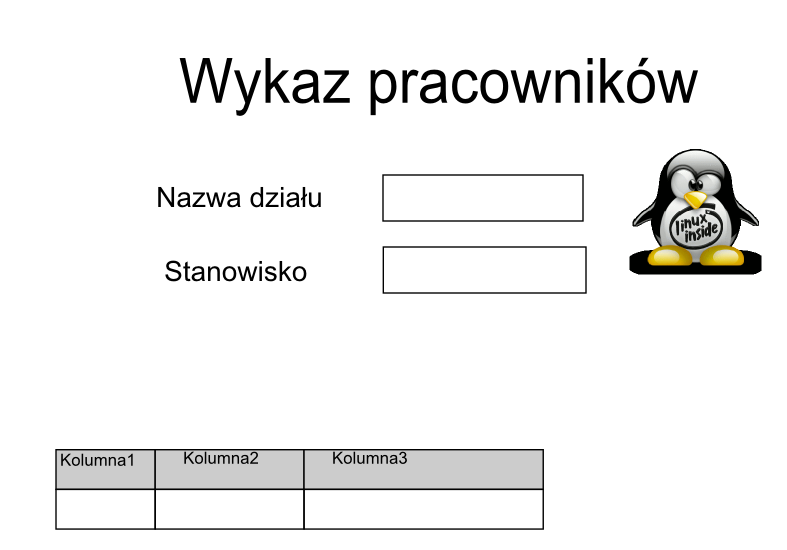
\includegraphics[scale=0.8]{sampleLayout}
\caption{Testowy wzorzec wyglądu raportu}
\label{img:sampleLayout}
\end{figure}

\subsection{Dane testowe} \label{test:data}
W celu prezentacji raportu typu \emph{master-detail} został wykorzystany związek jeden-wiele występujący między departamentami spółki, a pracownikami w nich zatrudnionymi. Przykład danych prezentujących ten związek był przedstawiony na listingu \ref{rap:complete} w rozdziale \ref{solution:data}.


\subsection{Realizacja w \emph{ApEx}} \label{test:apex}
Pierwszym krokiem do zaprezentowania rozwiązania jest utworzenie raportu interaktywnego. Na rysunku \ref{img:raport_ir_dane} zaprezentowane są kolumny wybrane do demonstracji. Istotne jest upewnienie się, że na raporcie będzie możliwe skorzystanie z menu \emph{\textbf{Actions}} oraz zawartej w nim opcji \emph{\textbf{Control Break}}, co jest konfigurowalne w szczegółach regionu z raportem interaktywnym. 

\begin{figure}[h]
\centering
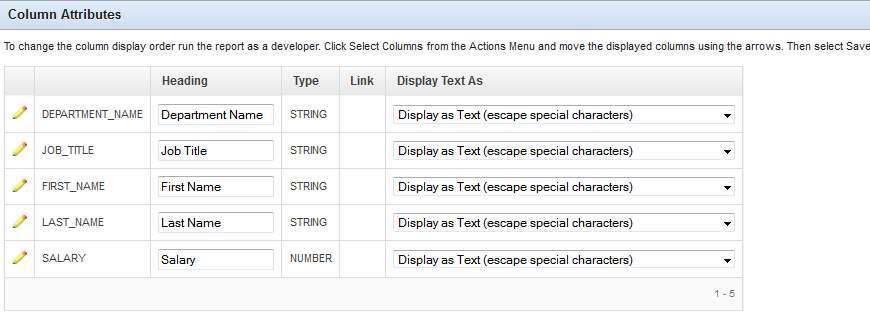
\includegraphics[scale=0.7]{ir_dane}
\caption{Kolumny wybrane do prezentacji raportu}
\label{img:raport_ir_dane}
\end{figure}


Następnym krokiem jest dodanie do strony dodatkowego elementu (\emph{\textbf{Items}}) typu \emph{\textbf{Hidden}}. W ustawioniach elementu musi być wybrana opcja umożliwiająca jego modyfikację na stronie (atrybut \emph{\textbf{Session State Protection}} ustawiony na \emph{\textbf{false}}). Element ten będzie służył do przechowywania nazw kolumn, które zostały wykorzystane do utworzenia grup danych za pomocą wbudowanej w \emph{ApExa} opcji \emph{\textbf{Control Break}}.  Rysunek \ref{img:final} przedstawia przykład grupy danych utworzonej za pomocą opcji \emph{\textbf{Control Break}}.



Kolejnym krokiem jest utworzenie w sekcji \emph{\textbf{Shared Components}} zapytań SQL oraz wzorca dla raportu. Przykładowe zapytanie zostało przedstawione na rysunku \ref{img:query}. Format nazwy zapytania stanowi niezbyt elegancki sposób rozwiązania pewnego problemu. Otóż, specyfikacja \emph{XSLT} nie zezwala na wykorzystanie wartości zmiennych jako selektora do pobierania danych, dlatego zostały utworzone zapytania i wzorce wyglądu raportu dla każdej kombinacji kolumn, dla której będzie generowany raport \emph{master-detail}. Zastosowanie zostanie zaprezentowane w dalszej części rozdziału. 

\begin{figure}
\centering
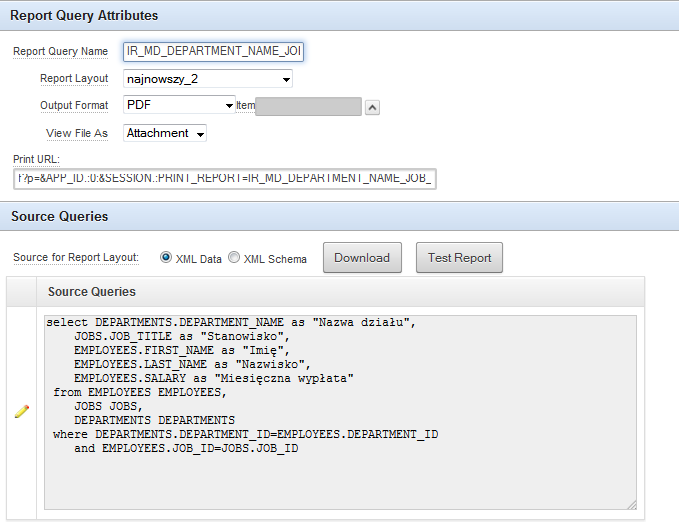
\includegraphics[scale=0.9]{query}
\caption{Przykładowe zapytanie \emph{SQL} pobierające dane testowe}
\label{img:query}
\end{figure}

W celu praktycznego zastosowania do strony został dodany przycisk. Wskutek jego kliknięcia wykonuje się dynamiczna akcja, w ramach której odbywają się dwie czynności. Pierwsza to wykonanie kodu \emph{\textbf{PL/SQL}}. Konfiguracja akcji jest przedstawiona na rysunku \ref{img:plsqlaction}. W ramach tej akcji z bazy danych ładowane są kolumnu użyte w funkcji \emph{\textbf{Control Break}}. Następnie wczytany łańcuch znaków jest podstawiany do ukrytego elementu strony, a jego stan jest zapamiętywany w sesji. \textbf{\emph{P10\_COLUMNS}} to nazwa ukrytego elementu strony. 

Druga akcja to wykonanie kodu \emph{\textbf{JavaScript}}. Wykonywany kod jest przedstawiony na listingu \ref{printjs}. Powoduje on odczytanie z ukrytego elementu strony łańcucha znaków zawierającego nazwy kolumn, a następnie zbudowanie adresu \emph{URL} na podstawie jego zawartości. Na końcu wykonywane jest przekierowanie \emph{HTTP} co skutkuje wygenerowaniem raportu.

\begin{figure}
\centering
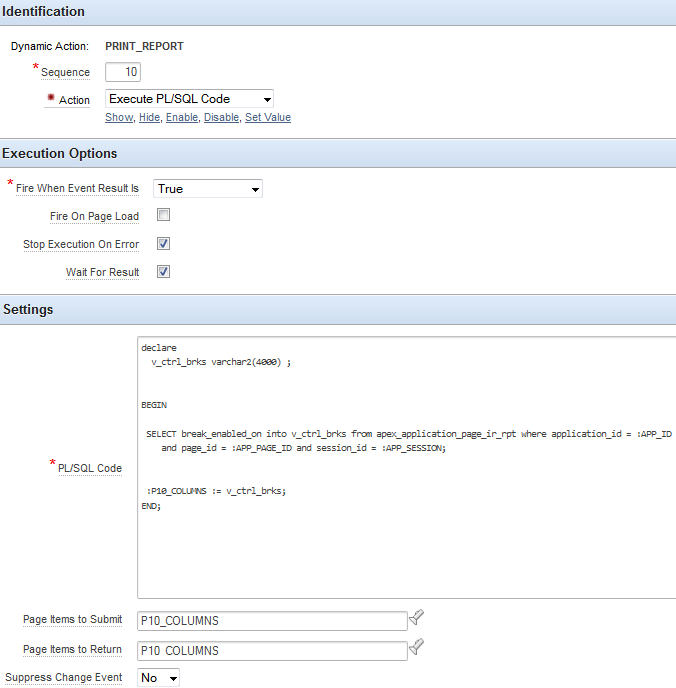
\includegraphics[scale=0.9]{plsql_act}
\caption{Konfiguracja akcji wykonującej kod PL/SQL}
\label{img:plsqlaction}
\end{figure}

\lstset{}
\begin{lstlisting}[frame=single,caption=Kod \emph{JavaScript} wykonywany po kliknięciu na przycisk,label=printjs]
var cols = $v('P10_COLUMNS');
var spl = cols.split(":");
var result = "";
var i = 0;
for( i= 0 ; i < spl.length ; i++ ) {
  if( spl[i] != '0' ) {
    if( i > 0 ) {
      result += '_'; 
    }
    result += s;
  }
}
var url = 'f?p=&APP_ID.:0:&SESSION.:PRINT_REPORT=IR_MD_' + result; 
window.location.href = url;

\end{lstlisting}



\begin{figure}[h]
\centering
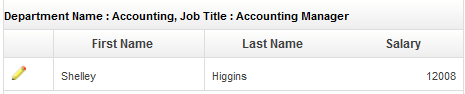
\includegraphics[scale=0.8]{final_screen}
\caption{Przykład grupy danych widocznej na raporcie interaktywnym}
\label{img:final}
\end{figure}


\subsection{Uzyskane wyniki} \label{test:result}
W wyniku uruchomienia przygotowywanego w ramach pracy narzędzia utworzone zostały trzy pliki, które należy wkleić do \emph{ApExa} w odpowiednie sekcje wzorca wyglądu raportu. Wynikowe pliki są nazwane tak, że nie pozostawiają wątpliwości co do tego, w której sekcji powinna znaleźć się poszczególna transformacja. Dokładne omówienie zawartości plików wyjściowych znajduje się w dodatku \ref{app:output}.

Efekt wydrukowania raportu składającego się z przedstawionych danych i wzorca wyglądu raportu oraz przy zastosowaniu zaprezentowanej konfiguracji znajduje się na rysunku \ref{img:wynikowy}, zawierającym pierwszą stronę wynikowego raportu. W tym przypadku jako \emph{master} zostały przyjęte: dział, w którym pracuje pracownik oraz zajmowane przez niego stanowisko. W tym przypadku została zastosowana kolumna o stałej szerokości. 

%wynikowy raport
\begin{figure}
\centering
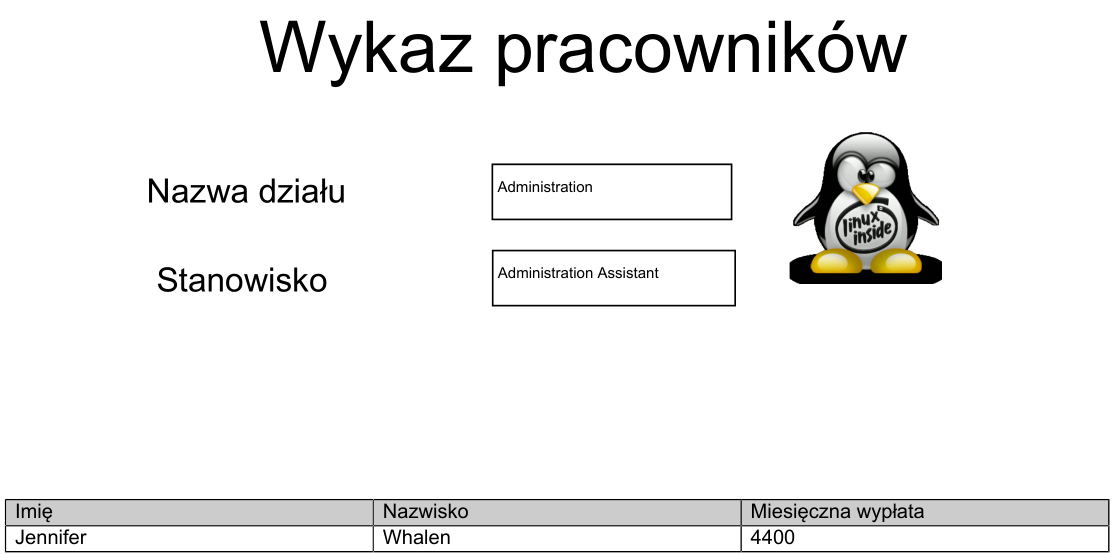
\includegraphics[scale=0.5,angle=90]{test-md}
\caption{Wynikowy raport typu \emph{master-detail}}
\label{img:wynikowy}
\end{figure}


\clearpage


\section{Wnioski i podsumowanie}
\emph{Oracle Application Express} to dość zaawansowane narzędzie umożliwiające sprawne tworzenie zarówno gotowych aplikacji, jak i raportów. Przy wykorzystaniu zewnętrznego narzędzia, możliwe jest również tworzenie raportów w formacie \emph{PDF} przeznaczonych do wydruku. W tym celu dane w formacie XML muszą zostać przekształcone do postaci XSL-FO. Przekształcenie to wykonuje się z wykorzystaniem XSLT, jednak jego wykorzystanie jest kłopotliwe w przypadku ręcznego programowania, gdyż wszelkie zmiany wyglądu raportu pociągają za sobą konieczność sporządzenia nowego arkusza transformacji XSLT.

Wsparcie \emph{ApEx'a} autorskim narzędziem rozwiązuje ten problem. Zastosowanie narzędzia w znacznym stopniu ogranicza konieczność stosowania wiedzy eksperckiej do sprawnego i wygodnego tworzenia raportów -- końcowy użytkownik nie musi znać standardu XSLT, a jedynie wkleić wygenerowane transformacje w odpowiednie sekcje. Dodatkowo samo tworzenie wzorca wyglądu raportu sprowadza się raczej do wykorzystania zdolności plastycznych, niż kompetencji technicznych.

Ponadto przy wykorzystaniu proponowanego rozwiązania dane są odseparowane od wzorca wyglądu raportu, a powiązanie między nimi jest realizowane za pomocą odpowiednich transformacji XSLT, co umożliwia użycie jednego faktycznego wzorca dla różnych danych.  

Kolejną cechą jest duża elastyczność stworzonego rozwiązania - dzięki wykorzystaniu pewnych cech \emph{ApExa} część parametrów raportu jest określana automatycznie, co zwiększa odporność na zmiany zestawu danych prezentowanych na raporcie. 

Nie bez znaczenia dla potencjalnej organizacji wykorzystującej narzędzie jest również fakt, że wszystkie wykorzystane standardy i technologie są darmowe. 

\bigskip
Środowisko tworzące system raportowy składa się z:
\begin{itemize}
	\item bazy danych Oracle wraz z Application Express,
	\item narzędzia do wydruków Apache Formatting Objects Processor,
	\item autorskiego narzędzia tworzącego arkusze XSLT przekształcające dane w formacie XML do postaci XSL-FO, co umożliwia ich wydruk w PDF za pomocą FOP.
\end{itemize}

\newpage

\begin{thebibliography}{9}

\bibitem{1} Bara George, \emph{Oracle APEX Reporting Tips \& Tricks}, Lulu.com, 2013,\\ISBN 978-1-291-41310-6
\bibitem{2} Garcia-Molina Hector, \emph{Systemy baz danych}, Wydanie II, Helion, 2011,\\ ISBN 978-83-246-3303-6
\bibitem{3} Creating Custom PDF Reports with Oracle Application Express and the APEX Listener, Oracle, Dostępny w internecie:\\http://www.oracle.com/technetwork/developer-tools/apex/learnmore/custom-pdf-reports-1953918.pdf
\bibitem{4} PDF Printing in Application Express, Oracle, Dostępny w internecie: \\http://www.oracle.com/technetwork/testcontent/configure-printing-093060.html
\end{thebibliography}
\newpage


\appendix
%włączanie usług sieciowych w oraklu
\section{Konfiguracja usług sieciowych po stronie bazy danych} \label{app:conf_db}
\begin{enumerate}
\item Uruchomienie klienta bazy danych, np. \emph{\textbf{SQL Developera}}.
\item Wykonanie skryptu SQL zawartego na listingu \ref{app:network}.

\lstset{language=SQL}
\begin{lstlisting}[frame=single,caption=Skrypt PL/SQL włączający usługi sieciowe w bazie danych,label=app:network]
DECLARE
  ACL_PATH  VARCHAR2(4000);
BEGIN
  SELECT ACL INTO ACL_PATH FROM DBA_NETWORK_ACLS
   WHERE HOST = 'localhost' AND LOWER_PORT IS NULL 
    AND UPPER_PORT IS NULL;
   
  IF DBMS_NETWORK_ACL_ADMIN.CHECK_PRIVILEGE
   (ACL_PATH, 'APEX_040200', 'connect') IS NULL THEN
      DBMS_NETWORK_ACL_ADMIN.ADD_PRIVILEGE(ACL_PATH,
     'APEX_040200', TRUE, 'connect');
  END IF;
  
EXCEPTION
  WHEN NO_DATA_FOUND THEN
  DBMS_NETWORK_ACL_ADMIN.CREATE_ACL
   ('local-access-users.xml',
    'ACL that lets users to connect to localhost',
    'APEX_040200', TRUE, 'connect');
  DBMS_NETWORK_ACL_ADMIN.
   ASSIGN_ACL('local-access-users.xml','localhost');
END;
/
COMMIT;
\end{lstlisting}

Skrypt ten sprawdza, czy została utworzona lista kontroli dostępu (\emph{Access Control List}) dla wskazanego hosta, w tym wypadku jest to \emph{\textbf{localhost}}. Jeśli taka lista już istnieje, to jest do niej dodawane uprawnienie dla użytkownika \emph{\textbf{APEX\_040200}}. Jeśli jednak taka lista nie istnieje, wtedy jest ona tworzona i przypisywana do wskazanego hosta.

\end{enumerate}
\newpage
%Stawianie APEX Listener
\section{Instalacja \emph{APEX Listener} i konfiguracja wbudowanego \emph{FOP}} \label{app:conf_fop}
\begin{enumerate}
\item Skonfigurowanie ustawień \emph{APEX Listenera}

Wykonuje się to poprzez uruchomienie wiersza poleceń i przejście do katalogu, w którym znajduje się archiwum \emph{\textbf{apex.war}}. Następnie należy wykonać komendę zawartą na listingu \ref{app:command}. 

\lstset{language=XML}
\begin{lstlisting}[frame=single,caption=Komenda służąca do konfiguracji \emph{APEX Listenera},label=app:command]
java -jar apex.war
\end{lstlisting}

Wskutek uruchomienia polecenia zostaniemy zapytani o dane dostępowe bazy danych, hasło użytkownika \emph{\textbf{APEX\_PUBLIC\_USER}} oraz ścieżkę pod którą chcemy przechowywać konfigurację. 

\item{Umożliwienie własnej konfiguracji wbudowanego \emph{FOP}}
Należy przejść do katalogu a konfiguracją \emph{APEX Listenera} wskazaną w poprzednim punkcie. Następnie do pliku \emph{default.xml} dodać dwa wpisy zawarte na listingu \ref{app:conf_fop_lst}, gdzie \textbf{\emph{\textless fop\_conf\textgreater}} to dowolnie wybrana przez nas ścieżka.

\lstset{language=XML}
\begin{lstlisting}[frame=single,caption=Wpisy do zawarcia w konfiguracji \emph{APEX Listenera},label=app:conf_fop_lst]
<entry key="misc.enableOldFOP">true</entry>
<entry key="fop.configfile"><fop_conf>\fop.xml</entry>
\end{lstlisting}

\item Konfiguracja czcionek dla \emph{FOP}
W przypadku nie wykonania tego kroku FOP skorzysta z podstawowych czcionek dysponujących ograniczonym zbiorem znaków. Jeśli chcemy wykorzystywać w raporcie znaki narodowe, należy dodać czcionkę \emph{True Type} zawierającą je. Zwykle w systemie operacyjnym występują już takie czcionki, trzeba jednak wskazać FOP ich lokalizację. W pliku odpowiadającym ścieżce podanej w poprzednim punkcie należy zamieścić instrukcje zawarte na listingu \ref{app:fop_font}. 

\lstset{language=XML}
\begin{lstlisting}[frame=single,caption=Konfiguracja czcionek dla \emph{FOP},label=app:fop_font]
<fop>
 <strict-configuration>true</strict-configuration>
 <renderers>
  <renderer mime="application/pdf">
   <fonts>
    <directory><font_path></directory>
   </fonts>
  </renderer>
 </renderers>
</fop>
\end{lstlisting}

Instrukcja \emph{\textbf{renderer mime="application/pdf"}} oznacza, że konfiguracja obowiązuje tylko przy tworzeniu pliku w formacie \emph{PDF}. \emph{\textbf{\textless font\_path\textgreater}} to ścieżka, pod którą znajdują się czcionki, z kolei instrukcja \emph{\textbf{\textless directory\textgreater}} powoduje zarejestrowanie dla \emph{FOP} wszystkich czcionek zawartych pod wskazaną ścieżką. Alternatywą jest wykorzystanie opcji \emph{\textbf{\textless auto-detect\textgreater}}, która powoduje zarejestrowanie dla \emph{FOP} wszystkich czcionek zainstalowanych w systemie operacyjnym.

\item Uruchomienie \emph{APEX Listenera} na kontenerze serwletów \emph{Apache Tomcat}

Można to zrobić poprzez skopiowanie archiwum \textbf{\emph{apex.war}} do podkatalogu \textbf{\emph{webapps}} instalacji \emph{Tomcata}, a następnie uruchomienie za pomocą skryptu znajdującego się w podkatalogu \textbf{\emph{bin}} o nazwie \textbf{\emph{catalina.sh}} lub \textbf{\emph{catalina.bat}} w zależności od systemu operacyjnego.

Alternatywnie, można najpierw uruchomić \emph{Tomcata} i za pomocą przeglądarki WWW uruchomić stronę \textbf{\emph{http://\textless host\textgreater :\textless port\textgreater/manager/}} i w sekcji \emph{\textbf{WAR file to deploy}} skorzystać z opcji \emph{\textbf{Przeglądaj}}.

\end{enumerate}
\newpage

%Inkscape conf
\section{Przygotowanie programu \emph{InkScape}} \label{app:inkscape}
\begin{enumerate}
\item Instalacja

W zależności od wybranej wersji wymaga to uruchomienia instalatora lub po prostu rozpakowania skompresowanego archiwum z programem.

\item Pobranie wtyczki \emph{Inkscape Table Support}.

Wtyczkę można pobrać z oficjalnej strony projektu \emph{\textbf{inkscape-tables}} znajdującej się na platformie \emph{\textbf{Sourceforge.net}} będącej hostingiem dla projektów \emph{Open Source}.

\item Instalacja wtyczki

Należy wypakować pobrane archiwum z wtyczką, a następnie wejśc do podkatalogu \emph{\textbf{modules}} wypakowanego pliku. Faktyczna instalacja wtyczki polega na skopiowaniu wszystkich plików z rozszerzeniami \emph{\textbf{.py}} oraz \emph{\textbf{.inx}} do katalogu \emph{\textbf{\textless inkscape\_dir\textgreater /share/extensions}}, gdzie \emph{\textbf{\textless inkscape\_dir\textgreater}} to katalog, w którym został zainstalowany \emph{Inkscape}.

\item Weryfikacja

W celu weryfikacji poprawności instalacji dodatku należy uruchomić program \emph{Inkscape}. Jeśli proces został wykonany poprawnie, to po kliknięciu na \emph{\textbf{Extension}} na górnym pasku programu w liście rozwijanej powinna być widoczna pozycja \emph{\textbf{Table}}.

\newpage
\end{enumerate}

%Out toola
\section{Pliki wyjścioweg przygotowanego narzędzia} \label{app:output}
\emph{\textbf{suffix}} w poniższych nazwach oznacza sufiks wybrany przez użytkownika podczas uruchomienia narzędzia.
\begin{itemize}
	\item \emph{\textbf{page\_suffix.xsl}} -- w tym pliku zawarta jest transformacja dla szablonu strony. Na widoku wzorca wyglądu raportu w \emph{ApExie} należy wkleić jego zawartość w sekcji \emph{\textbf{Page Template}}. W pliku tym zawarte są wartości atrybutów elementów występujących w raporcie. Ponadto transformacja w nim zawarta łączy pozostałe transformacje w całość.
	\item \emph{\textbf{header\_suffix.xsl}} --w tym pliku zawarta jest transformacja dla szablonu komórki nagłówka tabeli. Na widoku wzorca wyglądu raportu w \emph{ApExie} należy wkleić jego zawartość w sekcji \emph{\textbf{Report Column Heading}}. Transformacja zawarta w tym pliku tworzy pojedynczą komórkę nagłówka tabeli na podstawie nazwy określonej dynamicznie przez \emph{ApExa} w trakcie tworzenia wydruku. 
	\item \emph{\textbf{column\_suffix.xsl}} -- w tym pliku zawarta jest transformacja dla szablonu komórki ciała tabeli. Na widoku wzorca wyglądu raportu w \emph{ApExie} należy wkleić jego zawartość w sekcji \emph{\textbf{Column Template}}. Transformacja zawarta w tym pliku tworzy pojedynczą komórkę tabeli.
\end{itemize}

\end{document}

